\documentclass[11pt,a4paper]{report}

\usepackage{polski}
\usepackage[utf8]{inputenc} 
\usepackage{a4wide}
\usepackage{tabularx}
\usepackage{lastpage}
\usepackage{fancyhdr}
\usepackage{graphicx}

%strona tytułowa
\begin{titlepage}
\title{\Huge Specyfikacja Implementacyjna}
\author{Daniel Ślusarczyk i Jakub Łaba}
\date{10.03.2021}
\end {titlepage}

\renewcommand{\footrulewidth}{0pt}
\begin{document}
\maketitle

% zmiana numeracji sekcji 0.X -> X
\renewcommand*\thesection{\arabic{section}} 

\begin{abstract}
Dokument stanowi szczegółowy opis projektu "The Game of Life" oraz związaną z nim implementację. Zawiera informacje o użytych metodach, środowisku programu,
podziale na moduły i sposobie działania.
\end{abstract}

%Numeracja stron
\pagestyle{fancy}
\fancyhf{}
\rfoot{Strona \thepage \hspace{1pt} z \pageref{LastPage}}
\setcounter{page}{0}

% spis treści bez numeracji stron
\fancypagestyle{plain}
{
\fancyhead{} 
\fancyfoot{} 
}
\thispagestyle{empty} 
\tableofcontents 
\thispagestyle{empty}
\newpage

\fancypagestyle{plain} 
{
\fancyhead{} 
\fancyfoot[C]{\thepage}
}

% pierwsza sekcja
\section{Cel Projektu (skrócona wersja z poprzedniego dokumentu)}\label{sec:tekst}
Program symuluje działanie automatu komórkowego Johna Conwaya - Grę w Życie (ang. "The Game of Life").\\
Na prostokątnej planszy znajdują się komórki żywe oraz martwe.\\
"Życie" na planszy toczy się przez określoną liczbę generacji, które są rozdzielone dyskretnymi odstępami czasowymi.\\
W każdej generacji komórki:\\
	-Żywe: pozostają żywe w kolejnej generacji jeżeli posiadają dokładnie 2 lub 3 żywych sąsiadów, w każdym innym przypadku umierają\\
	-Martwe: ożywają w kolejnej generacji jeżeli posiadają dokładnie trzech żywych sąsiadów, w przeciwnym przypadku pozostają martwe\\


% druga sekcja
\section{Środowisko Powstawiania Programu}\label{sec:teskt}
\begin{tabularx}{\textwidth}{  X|Xl  }
\hline
			System operacyjny		&Windows Subsystem for Linux, Ubuntu 20.04\\
\hline
			Język programowania	&C\\
\hline
			Kompilator			&gcc 9.3.0\\
\end{tabularx}
\newpage

% trzecia sekcja
\section{Diagram Modułów}\label{sec:teskt}
Program składa się z dwóch modułów - tgol\_file oraz tgol\_evo.
Każdy z modułów składa się z dwóch plików - nagłówkowego oraz pliku źródłowego C.
Poza tym program zawiera plik tgol\_main.c, zawierający funkcję main całego programu.
\begin{figure}[htbp]
\centerline{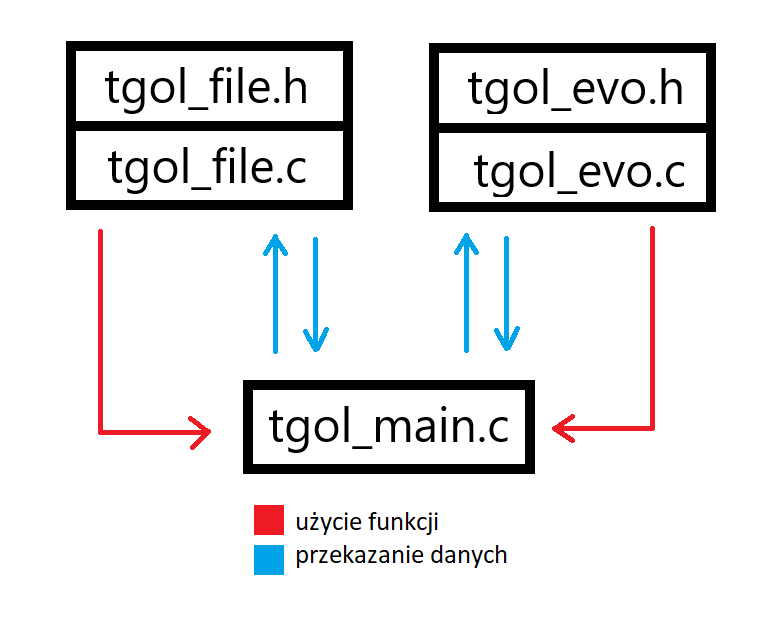
\includegraphics{diagram_modułów.png}}
\label{fig}
\end{figure}


% czwarta sekcja
\section{Opis Modułów i Funkcji}\label{sec:teskt}
Moduł tgol\_file zawiera funkcje odpowiadające za obsługę plików w obrębie programu - wczytywanie, przetwarzanie danych oraz tworzenie nowych plików przez program.
Moduł tgol\_evo zawiera funkcje odpowiadające za ewolucję komórek na planszy.
Moduły tgol\_file oraz tgol\_evo są od siebie niezależne (nie korzystają nawzajem ze swoich funkcji i nie przekazują bezpośrednio między sobą danych), plik tgol\_main.c jest zależny od obydwu modułów.


% piąta sekcja
\section{Struktura Danych}\label{sec:teskt}
Przeprowadzenie wszystkich generacji dla planszy wymaga przeanalizowania conajmniej N x M x L pól, gdzie:
	N-ilość wierszy planszy
 	M-ilość kolumn planszy
	L-ilość generacji
Dodatkowo znaczna większość komórek na planszy zawsze pozostoje martwa, więc na obliczenia wpływ miałby tylko ułamek ze wszystkich przechowywanych informacji o 
polach. Z tych powodów omawiane oprogramowanie zakłada użycie specjalnego formatu reprezentacji macierzy rzadkiej jaką jest CRS (z ang. compressed row storage), która
przechowuje wyłącznie informacje o niezerwowych elementach analizowanej planszy.
Zasada działania CRS:
Macierz rzadka wymiarów n x m jest reprezentowana przez dwa osobne jednowymiarowe wektory: col\_index, row\_index. Pierwszy z nich (col\_index) jest numerowany od 0 (pierwsza kolumna to kolumna 0) i odpowiada za przechowywanie w kolejności indeksów kolumn,
w których znajdują się niezerwowe wartości. Drugi (row\_index) - zawsze rozpoczyna się od 0 i jego wartościami są ilości niezerwowych elementów, które wystąpiły w  kolejnych wierszach.
\subsection{Przykład}
1 0 0 0
0 1 0 0
0 0 1 0
1 1 0 0
col\_index: [0 1 2 0 1]
row\_index: [0 1 2 3 5]

% szósta sekcja
\section{Sposób Wprowadzania Zmian i Przeprowadzania Testów}\label{sec:teskt}
Do wprowadzania zmian w projekcie używany jest system kontroli wersji git.
Program obsługuje wiele rodzajów błędów - testy zostaną przeprowadzone poprzez uruchomienie programu z odpowiednio spreparowanymi, niepoprawnymi argumentami wywołania i formatowaniem pliku wejściowego, tak aby otrzymać każdy z komunikatów błędów z osobna.
Z wyników testów będą tworzone zwięzłe raporty w postaci plików .txt i będą udostępniane całemu zespołowi za pośrednictwem gita.

% siódma sekcja
\section {Rozwiązanie Problemu Granicy Planszy}\label{sec:teskt}
Plansza będzie przechowywana w postaci informacji o macierzy, po której komórkach będzie iterować główna pętla programu.
Jeżeli komórka znajduje się na skraju macierzy, to co najmniej jedna z jej współrzędnych jest skrajna, tj. równa 0 lub o 1 mniejsza od szerokości (w przypadku współrzędnej x) lub wysokości (w przypadku współrzędnej y) macierzy.
Aby przy sprawdzaniu sąsiadów dookoła poszczególnych komórek uniknąć przekroczenia dozwolonego zakresu operatorami pętli, zakresy sprawdzania sąsiedztwa zostaną odpowiednio ograniczone dla skrajnych komórek.


\end{document}